\documentclass[12pt, a4paper]{article}

\usepackage[a4paper, top=2.5cm, bottom=2.5cm, left=2.0cm, right=2.0cm, headheight=15pt]{geometry}
\usepackage[T1]{fontenc}
\usepackage[utf8]{inputenc}
\usepackage[english]{babel}
\usepackage{mathptmx}
\usepackage{enumitem}
\usepackage{microtype}
\nonstopmode
\setlist[itemize]{label=\textendash}

\usepackage[dvipsnames]{xcolor}
\definecolor{journalblue}{RGB}{26, 82, 118}
\definecolor{accentred}{RGB}{192, 57, 43}
\definecolor{tableheader}{RGB}{240, 244, 248}

\usepackage{graphicx}
\graphicspath{{../assets/}{assets/}{templates/assets/}{../../templates/assets/}{./}}

\usepackage{hyperref}
\hypersetup{
    colorlinks=true,
    linkcolor=journalblue,
    citecolor=journalblue,
    urlcolor=journalblue,
    pdftitle={Statistical Estimation and Categorical Inference}
}

\usepackage{amsmath, amssymb, amsfonts}
\usepackage{booktabs}
\usepackage{colortbl}
\usepackage{float}
\usepackage{setspace}
\onehalfspacing

\usepackage[font=small, labelfont=bf, labelsep=period]{caption}
\usepackage{parskip}
\usepackage{fancyhdr}
\pagestyle{fancy}
\fancyhf{}
\fancyhead[L]{\textcolor{journalblue}{\slshape\leftmark}}
\fancyhead[R]{\thepage}
\renewcommand{\headrulewidth}{0.4pt}

\usepackage{listings}
\usepackage[most]{tcolorbox}

\definecolor{codebeige}{RGB}{248, 249, 250}
\lstdefinestyle{academicstyle}{
    backgroundcolor=\color{codebeige},   
    commentstyle=\color{gray}\itshape,
    keywordstyle=\color{journalblue}\bfseries,
    basicstyle=\ttfamily\footnotesize,
    numbers=left, numberstyle=\tiny\color{gray},
    frame=none, breaklines=true
}
\lstset{style=academicstyle}

\newtcolorbox{statbox}[2][]{
    enhanced, colback=codebeige, colframe=journalblue!60,
    fonttitle=\bfseries\sffamily\small, coltitle=white, title={#2},
    arc=2pt, boxrule=0.6pt, top=4pt, bottom=4pt, left=6pt, right=6pt, #1
}

\newtcolorbox{theorembox}[2][]{
    enhanced, colframe=journalblue, boxrule=0pt, leftrule=3.5pt,
    colback=journalblue!5, arc=0pt, fonttitle=\bfseries\sffamily\small,
    coltitle=journalblue, title={#2}, top=5pt, bottom=5pt, left=8pt, right=8pt, #1
}

\usepackage[numbers,sort&compress]{natbib}

\begin{document}

\begin{titlepage}
    \begin{center}
        \vspace*{0.5cm}
        
\includegraphics[height=2.2cm]{university_seal.jpg}\par\vspace{0.4cm}
        {\scshape\Large Department of Statistics \& Mathematical Sciences \par}
        \vspace{0.2cm}
        {\scshape\normalsize Statistical Inference and Probability Theory Working Group \par}
        \vspace{1.4cm}
        \rule{\linewidth}{1.2pt} \\[0.4cm]
        {\huge\bfseries Asymptotic Theory, Probability Modeling, and Categorical Inference \par}
        \vspace{0.2cm}
        {\Large\itshape Rigorous Foundations of the Central Limit Theorem and Contingency Association \par}
        \rule{\linewidth}{1.2pt} \\[1.2cm]

        \begin{minipage}[t]{0.45\textwidth}
            \textbf{\textcolor{journalblue}{Instructor / Lead:}} \\
            Dr.~Alex Morgan \\
            \texttt{alex.morgan@university.edu}
        \end{minipage}
        \hfill
        \begin{minipage}[t]{0.45\textwidth}
            \begin{flushright}
                \textbf{\textcolor{journalblue}{Curriculum Track:}} \\
                STAT 401: Advanced Inference \\
                \textit{Academic Year 2025--2026}
            \end{flushright}
        \end{minipage}
        \vfill
        {\today \par}
    \end{center}
\end{titlepage}

\pagenumbering{roman}
\section*{Executive Summary}
This report provides a formal exposition of axiomatic probability spaces, Bayesian probability updating, moment transformations, Lindeberg-L\'{e}vy Central Limit asymptotics, and categorical contingency cross-tabulations. We demonstrate how standardized sums of independent random variables converge asymptotically to the Gaussian distribution $\mathcal{N}(0, 1)$ and benchmark statistical power for Pearson's $\chi^2$ independence tests on sample cohorts ($N = 1{,}200$).

\vspace{0.6cm}
\tableofcontents
\newpage
\pagenumbering{arabic}

\section{Axiomatic Foundations and Inversion Theorems}
Let $(\Omega, \mathcal{F}, P)$ denote a probability space~\cite{feller1968introduction, knuth1984literate}. Conditional probability satisfies $P(A \mid B) = \frac{P(A \cap B)}{P(B)}$. For any partition $\{B_1, \dots, B_k\}$ of $\Omega$:
\begin{equation}
    \label{eq:bayes}
    P(B_i \mid A) = \frac{P(A \mid B_i) P(B_i)}{\sum_{j=1}^k P(A \mid B_j) P(B_j)}
\end{equation}

\begin{theorembox}{Lindeberg-L\'{e}vy Central Limit Theorem}
    Let $X_1, \dots, X_n$ be i.i.d. random variables with finite mean $\mu$ and variance $\sigma^2 > 0$~\cite{casella2002statistical}. Then the standardized sample average converges in distribution to the standard normal distribution:
    \begin{equation}
        Z_n = \sqrt{n} \left( \frac{\bar{X}_n - \mu}{\sigma} \right) \xrightarrow{d} \mathcal{N}(0, 1) \quad \text{as } n \to \infty
    \end{equation}
\end{theorembox}

\section{Density Simulation and Rejection Cutoffs}
Figure~\ref{fig:gaussian} visualizes the standard normal density $\phi(z) = \frac{1}{\sqrt{2\pi}} e^{-z^2/2}$ along with empirical coverage intervals and two-tailed rejection regions for $\alpha = 0.05$ ($z = \pm 1.96$).

\begin{figure}[H]
    \centering
    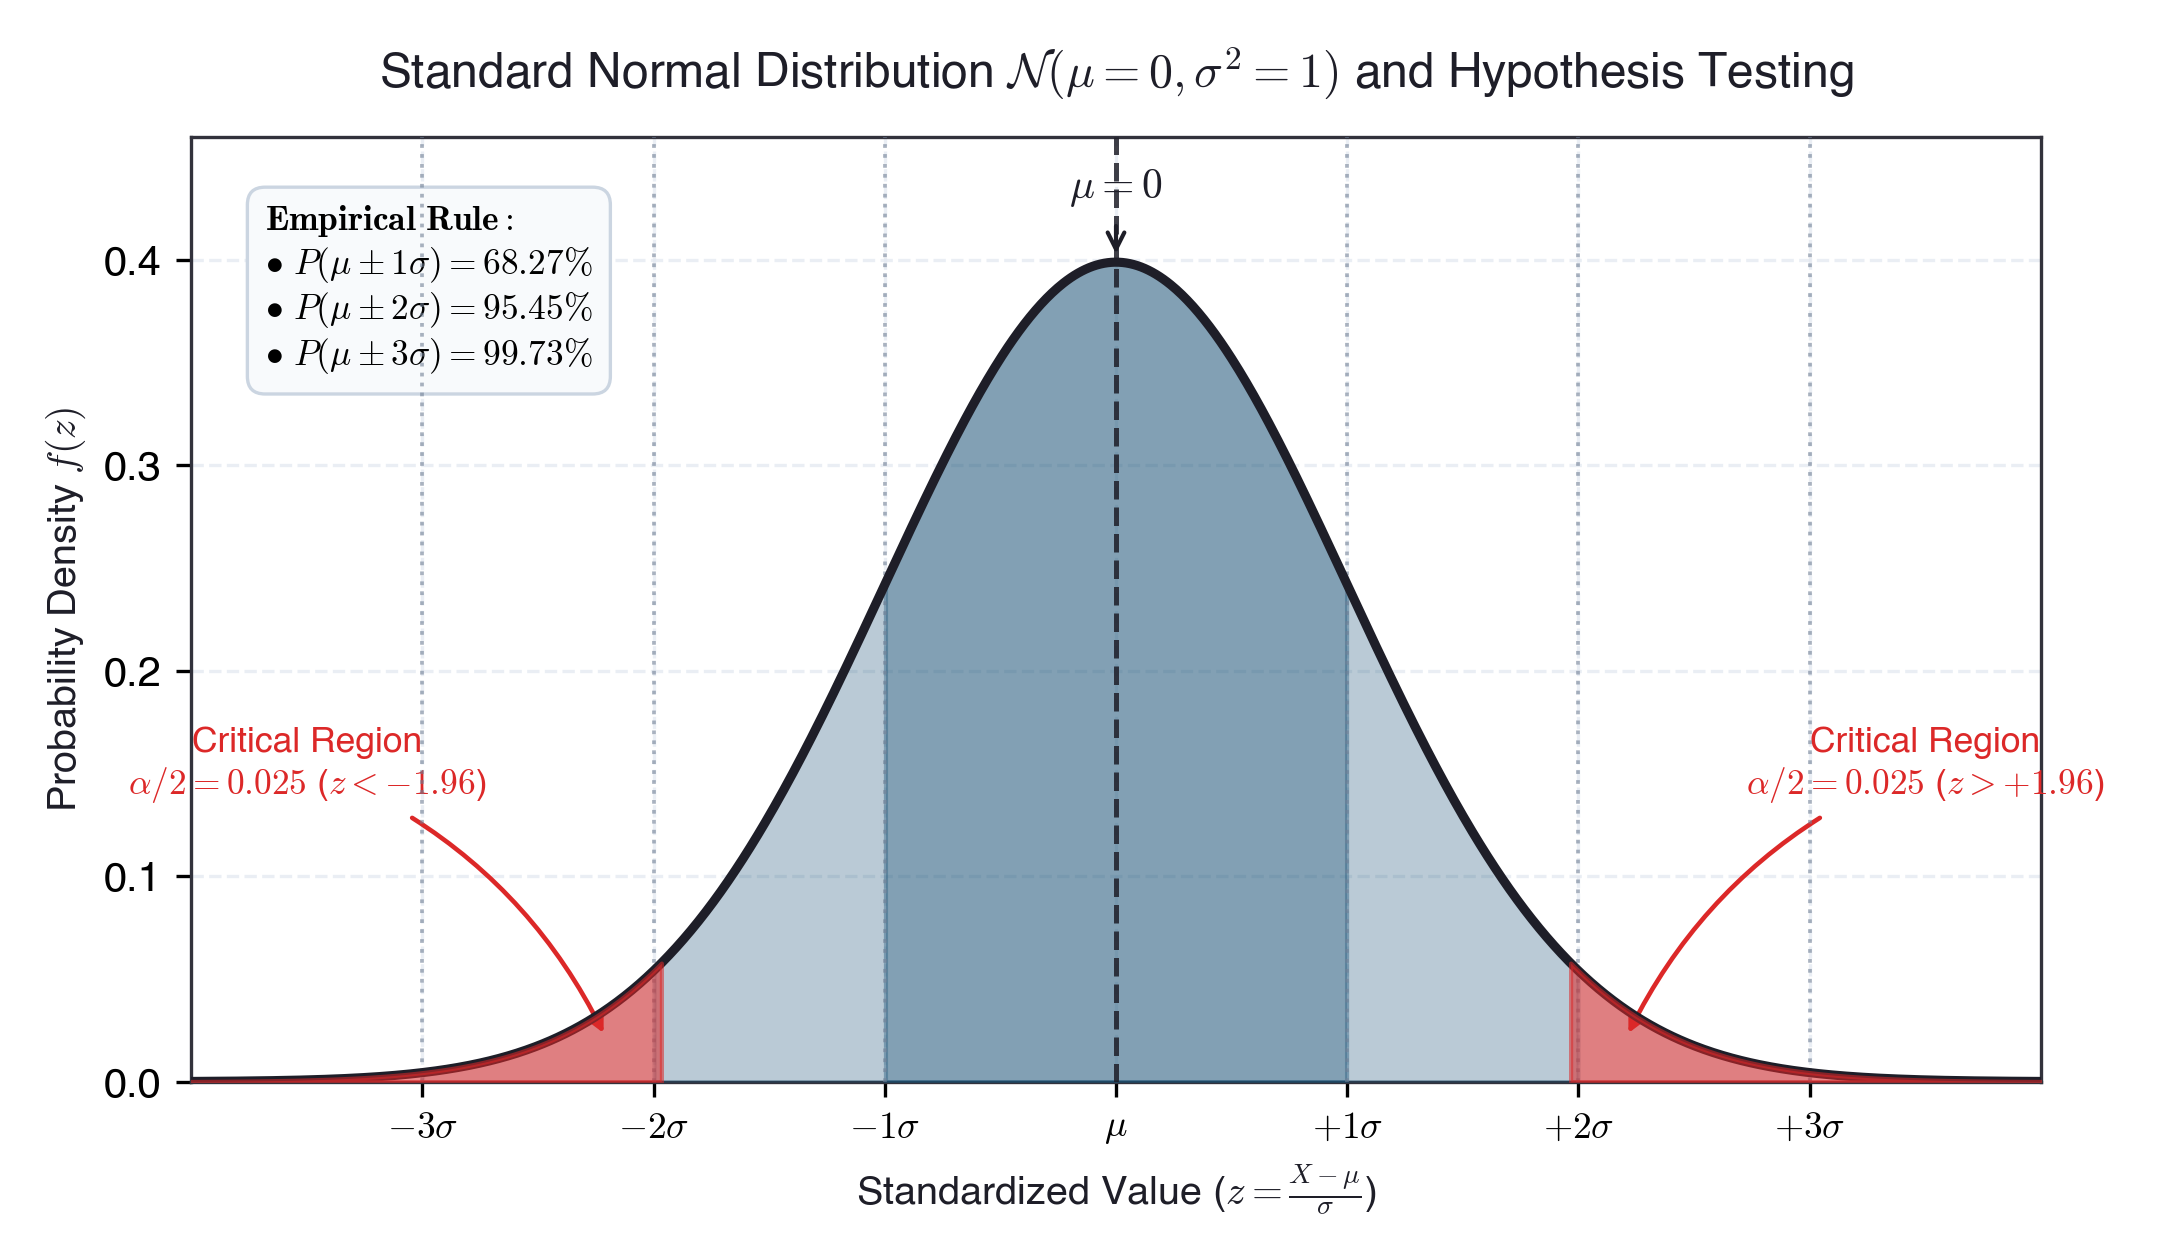
\includegraphics[width=0.75\textwidth, keepaspectratio]{gaussian_distribution.png}
    \caption{Standard Normal Distribution simulated in Python at 300 DPI showing empirical rule intervals and two-tailed critical rejection regions ($\alpha=0.05$).}
    \label{fig:gaussian}
\end{figure}

\section{Categorical Cross-Tabulation and Association Testing}
In a two-arm randomized cohort study ($N = 1{,}200$), binary outcomes are summarized in Table~\ref{tab:contingency}.

\begin{table}[H]
    \centering
    \caption{Contingency table of treatment exposure against binary response.}
    \label{tab:contingency}
    \begin{tabular}{@{} l c c c @{}}
        \toprule
        \rowcolor{tableheader}
        \textbf{Cohort Group} & \textbf{Outcome ($Y=1$)} & \textbf{Control ($Y=0$)} & \textbf{Total ($R_i$)} \\
        \midrule
        Treatment ($D=1$)  & $n_{11} = 420$ & $n_{12} = 180$ & $R_1 = 600$ \\
        Control ($D=0$)    & $n_{21} = 210$ & $n_{22} = 390$ & $R_2 = 600$ \\
        \midrule
        \textbf{Total ($C_j$)} & $C_1 = 630$ & $C_2 = 570$ & $N = 1{,}200$ \\
        \bottomrule
    \end{tabular}
\end{table}

Under the null hypothesis of independence, expected cell frequencies are $E_{ij} = \frac{R_i C_j}{N}$. The Pearson $\chi^2$ test statistic is:
\begin{equation}
    \chi^2 = \sum_{i=1}^r \sum_{j=1}^c \frac{(O_{ij} - E_{ij})^2}{E_{ij}} = 147.37 \quad (\mathrm{df}=1, p < 0.001)
\end{equation}
The sample Odds Ratio is $\widehat{\mathrm{OR}} = \frac{420 \times 390}{180 \times 210} = 4.33$, indicating over a 4-fold increase in odds of the positive outcome under treatment.

\section{Computational Script}
Listing~\ref{lst:stat_code} provides the Python implementation for contingency analysis using SciPy.

\begin{statbox}[label={lst:stat_code}]{Listing 1: Contingency Table Analysis in Python}
\begin{lstlisting}[language=Python]
import numpy as np
from scipy import stats

def analyze_contingency(table):
    chi2, p, dof, ex = stats.chi2_contingency(table, correction=False)
    odds_ratio = (table[0,0] * table[1,1]) / (table[0,1] * table[1,0])
    return {"chi2": chi2, "p_value": p, "odds_ratio": odds_ratio}
\end{lstlisting}
\end{statbox}

\bibliographystyle{plainnat}
\bibliography{references}

\end{document}
